\documentclass{beamer}

\usepackage{amsmath, amssymb}
\usepackage{tikz-cd}
\usepackage{xcolor}
\usepackage{graphicx}

\title{MAT222: Calculus II - Technique of Integration}
 \subtitle{7.8 Improper Integrals}

\author{\textbf{Miraj Samarakkody}}
\institute{Tougaloo College}
\date{Updated: \today}

\begin{document}

\begin{frame}
    \titlepage
\end{frame}


\begin{frame}{Introduction}
    
    \begin{block}{Definition}
        A \textbf{improper integral} is an integral that has one of the following properties:
        \begin{itemize}
            \item The interval of integration is infinite.
            \item The integrand is infinite at one or more points in the interval of integration.
        \end{itemize}
    \end{block}
\end{frame}

\begin{frame}{Type I - Infinite Intervals}
    Consider the infinite region \(S\) that lies under the curve \(y=1/x^2\), above the \(x-\)axis, and the right of the line \(x=1\). 

    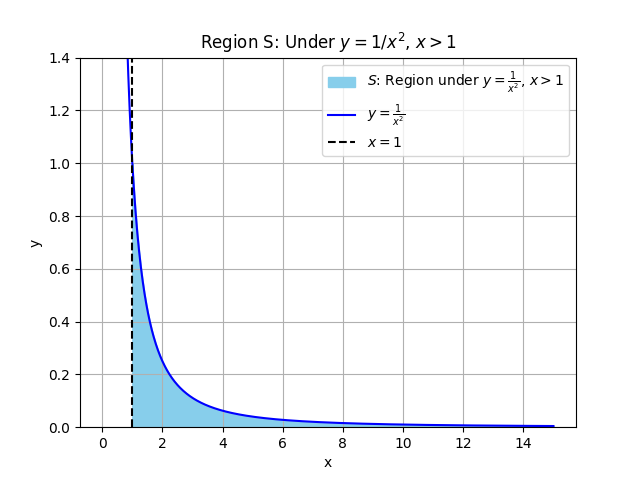
\includegraphics[scale=0.5]{figures/fig_2.png}
\end{frame}





\end{document}